\UseRawInputEncoding
\documentclass[12pt]{beamer}
\usecolortheme[named=red]{structure}

\usepackage[T1]{fontenc}
\usepackage[utf8]{inputenc}
\usepackage{lmodern}

\def\magyarOptions{defaults=hu-min}
\usepackage[magyar]{babel}
\usepackage[autostyle]{csquotes}
\DeclareQuoteStyle{magyar}{,,}{''}{>>}{<<}

%\usetheme{CambridgeUs}
\usepackage{epstopdf}
\usepackage{graphicx}
\usepackage{subcaption}
\usepackage{wrapfig}
\usepackage{media9}
\usepackage{amsmath}
\usecolortheme{beaver}
\usepackage{multicol}
\usepackage{siunitx}
\hypersetup{unicode=true}

\setbeamertemplate{enumerate items}[circle]
\setbeamertemplate{itemize items}[circle]
 
%Information to be included in the title page:
\title[Doktori téma]{Stochastic properties of\\dislocation motion and rearrangement\\{\small Investigated by cellular automata and experiments}}

\author[Tüzes]{Tüzes Dániel}
 
\institute[ELTE Fizika Doktori Iskola] % (optional)
{
  Anyagtudomány és szilárdtestfizika, Fizika Doktori Iskola, ELTE TTK
}

\date{Felelet a bírálatokra\\2019. május 3.}

\begin{document} 
\frame[plain]{\titlepage}
 
 
\section{Hartmann Péternek válasz}
\subsection{Megjegyzés}
\begin{frame}
\centering
\huge Válasz\\
\large Dr. Hartmann Péternek
\end{frame}
\begin{frame}
\frametitle{Ábrák jelölése fekete-fehérben}
\begin{figure}
\begin{subfigure}{0.49\textwidth}
\includegraphics[width=1\textwidth]{figs/strain_to_failure_vs_system_size.pdf}
\caption{Színesben}
\end{subfigure}
\begin{subfigure}{0.49\textwidth}
\includegraphics[width=1\textwidth]{figs/strain_to_failure_vs_system_size_bw.pdf}
\caption{Fekete fehérben}
\end{subfigure}
\end{figure}
A jelölők különböznek az alakzat formájában is.\\
A vonalak különböznek a szaggatás típusában is.
\end{frame}

\subsection{Korrelációs integrál}
\begin{frame}
\frametitle{Korrelációs integrál}
{\centering
\begin{figure}
\includegraphics[width=0.65\textwidth]{figs/corr_int.pdf}
\end{figure}
$C\left( r \right)$: hány lavina van $r$ távolságon belül.\\
\par}
[1]: Jérôme Weiss and David Marsan. Three-dimensional mapping of dislocation avalanches: clustering and space/time coupling. Science, 299(5603):89–92, 2003.
\end{frame}

\subsection{A rendezetlenség szerepe törésnél}
\begin{frame}
\frametitle{A rendezetlenség szerepe törésnél}
Saját hozzájárulás:
\begin{itemize}
\item A modell továbbfejlesztése
\item Szimulációk futtatása, eredmények összegyűjtése
\item Kiértékelőprogramok írása, futtatása
\item Eredmények ábrázolása, szöveges értelmezése
\item Cikk szerkezetének felépítése, első változat megírása
\end{itemize}
Társszerzők munkája
\begin{itemize}
\item Michael Zaiser: motiváció [2] és felismerés, szakirodalmi kontextus, eredmények értelmezése
\item Ispánovity Péter: aktivációs feszültség eloszlásából hogyan lehet jósolni a törés bekövetkeztét + ábra
\end{itemize}
[2]: Zoe Budrikis and Stefano Zapperi. Avalanche localization and crossover scaling in
amorphous plasticity. Phys. Rev. E, 88:062403, Dec 2013. doi: 10.1103/PhysRevE.
88.062403.
\end{frame}

\begin{frame}
\frametitle{A rendezetlenség szerepe törésnél}
Példa:
\begin{itemize}
\item Fémüvegek [3]
\item Fémhabok [4]
\end{itemize}
[3]: Christopher A Schuh, Todd C Hufnagel, and Upadrasta Ramamurty. Mechanical behavior of amorphous alloys. Acta Materialia, 55(12):4067–4109, 2007.

[4]: Zaiser M, Mill F, Konstantinidis A, Aifantis K (2013) Strain localization and strain propagation in collapsible solid foams. Mater Sci Eng A 567:38–45

\end{frame}

\section{Börzsönyi Tamásnak válasz}
\begin{frame}
\centering
\huge Válasz\\
\large Dr. Börzsönyi Tamásnak
\end{frame}

\begin{frame}
\frametitle{Feszültség-deformációs görbe + AE régi}
\begin{center}
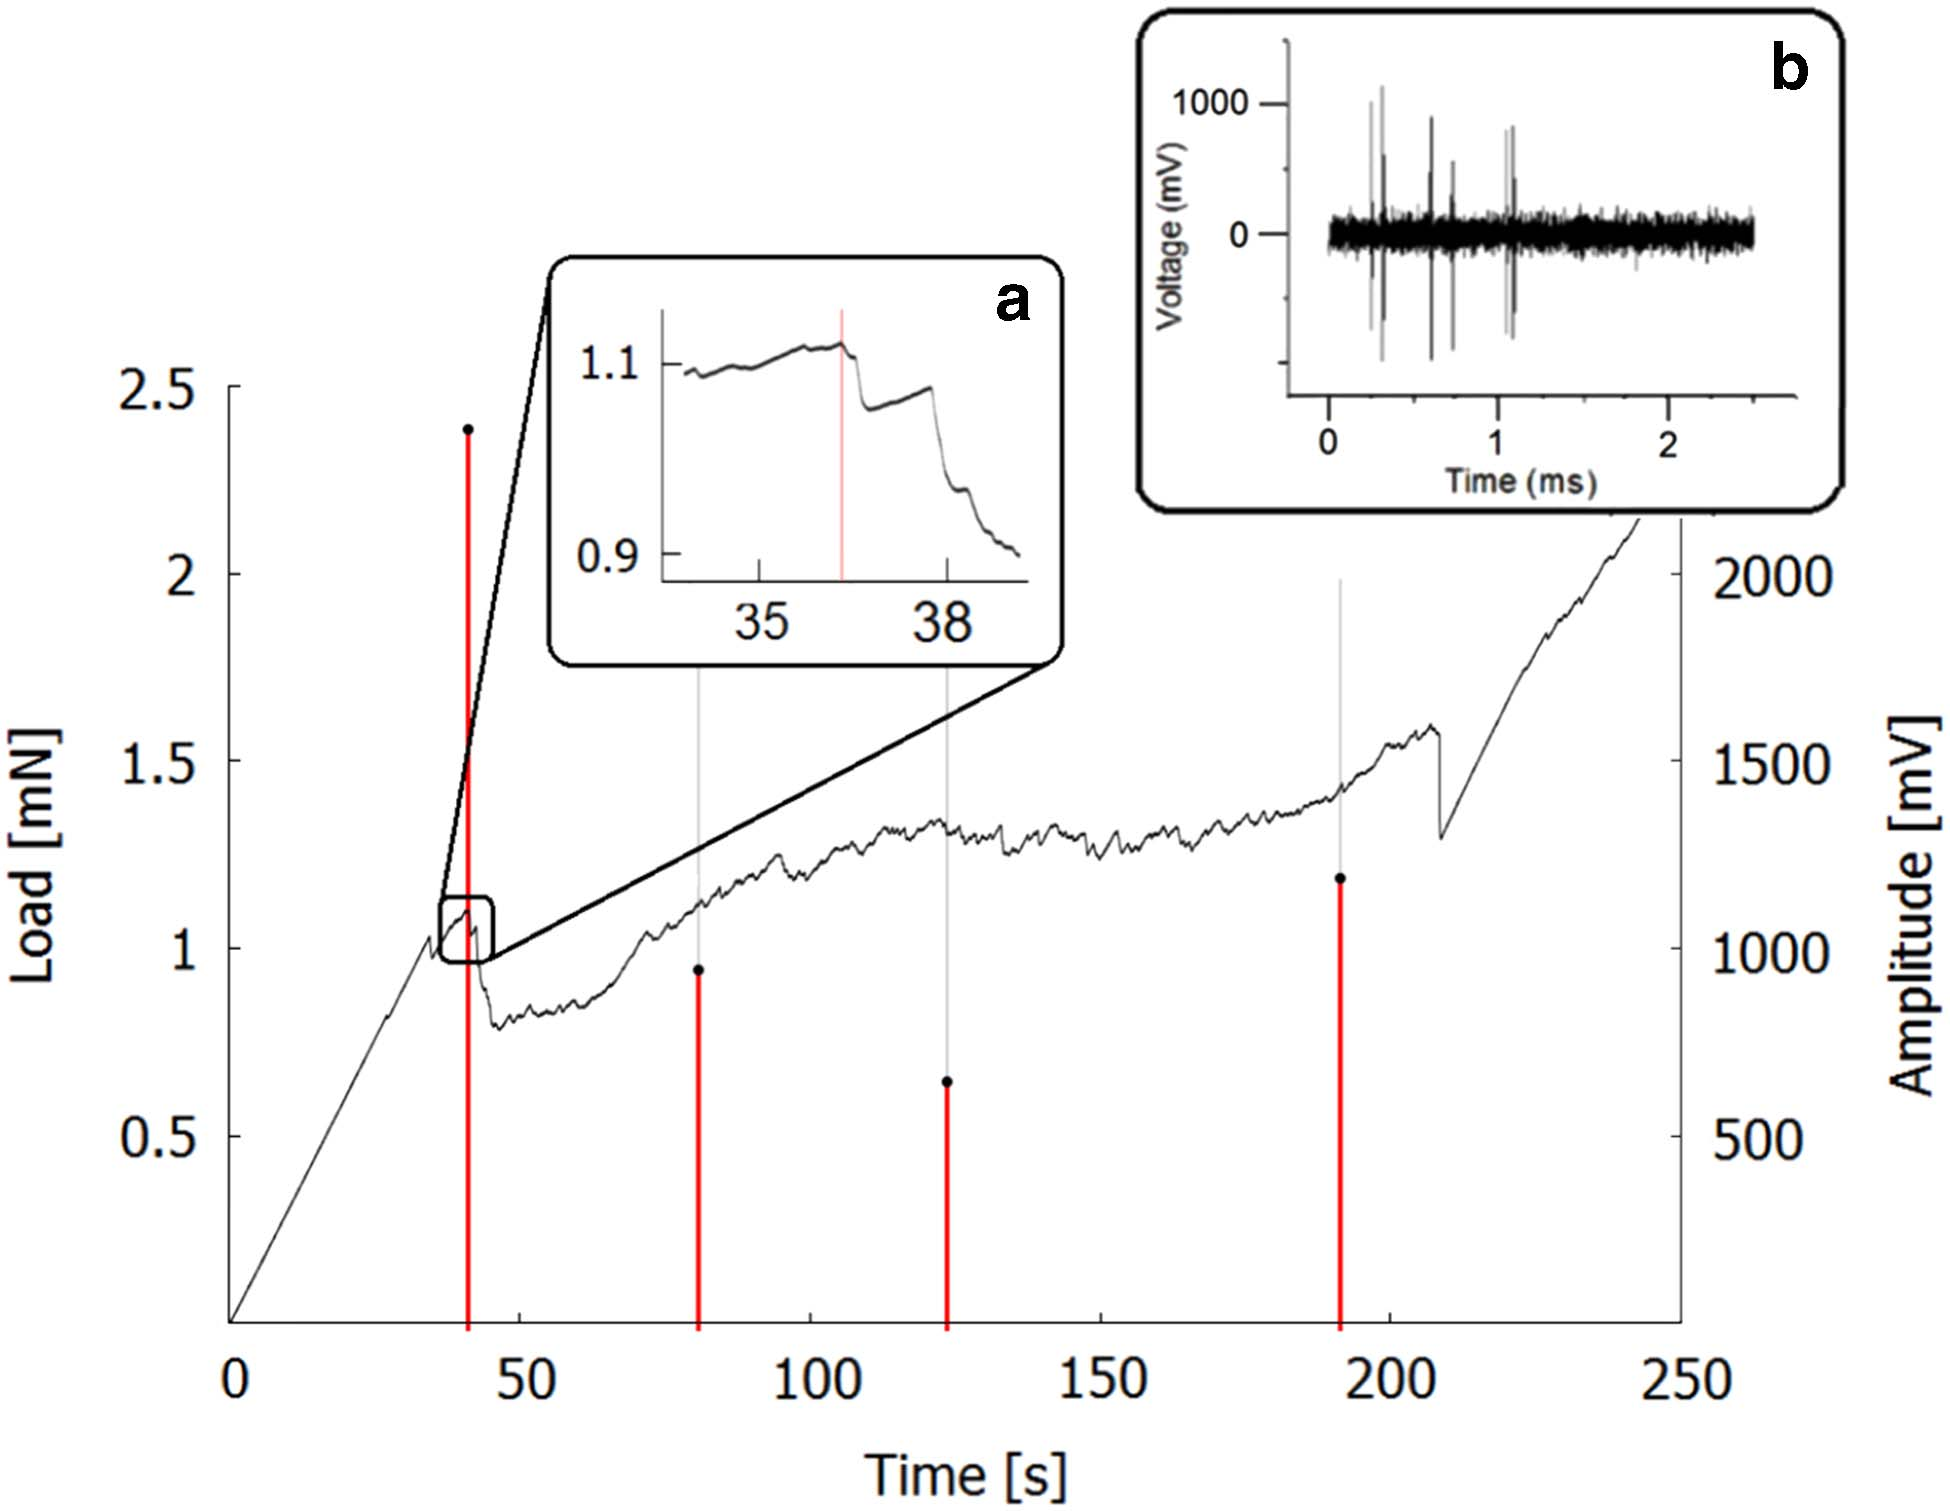
\includegraphics[width=0.8\textwidth]{figs/Micron-Scale_Deformation3.jpg} 
\end{center}
\end{frame}

\begin{frame}
\frametitle{Feszültség-deformációs görbe + AE új}
\begin{center}
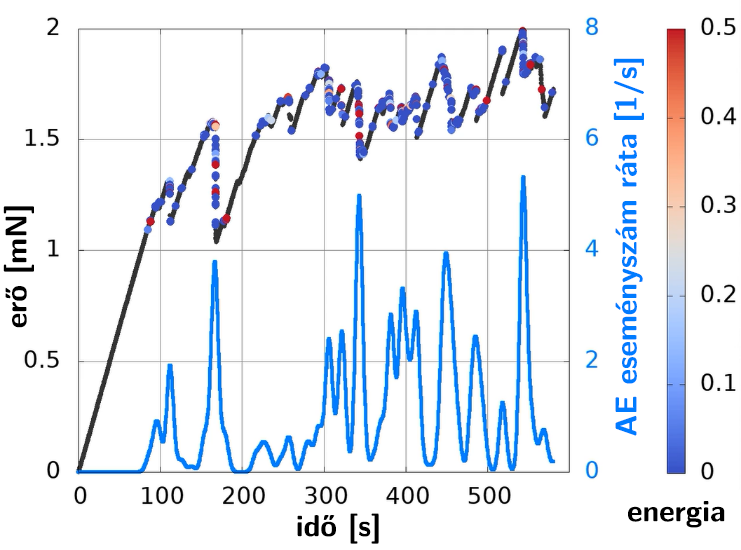
\includegraphics[width=0.8\textwidth]{figs/frame.png} 
\end{center}
\end{frame}
\begin{frame}
\frametitle{Feszültség-deformációs görbe + AE + in situ}
\begin{center}

\includemedia[label=insitu,
addresource=figs/output_correlated.mp4,
activate=pageopen,
passcontext,
flashvars={source=figs/output_correlated.mp4&loop=true}]{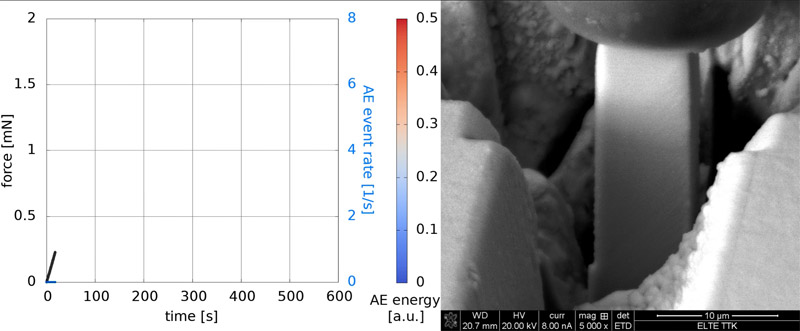
\includegraphics[width=1\textwidth]{figs/frame.jpg}}{VPlayer.swf}

\end{center}
\end{frame}

\end{document}

